\documentclass[11pt,a4paper]{article}

\usepackage{../../templates/style}

\begin{document}

\begin{problem}{Roboturtle}{standard input}{standard output}{1 second}{64 megabytes}


ในการควบคุมเต่ายนต์ตัวหนึ่ง ถ้าเราสามารถควบคุมเต่าตัวนี้ให้เคลื่อนที่ในแนวราบด้วยคำสั่ง \textbf{‘FD’ ‘RT’ ‘LT’ ‘BW’ }ซึ่งเป็นการกำหนดทิศทางการเดินทางไป ไปด้านหน้า หันด้านขวา หันด้านซ้าย และหันย้อนกลับ ตามลำดับ โดยแต่ละคำสั่งสามารถกำหนดระยะในการเคลื่อนที่ได้ ถ้าหากว่าจุดเริ่มต้นของเต่าอยู่ที่พิกัด $(0,0)$ มุ่งหน้าไปทางทิศตะวันออก \textbf{(E)} แล้วได้รับคำสั่งมาเป็นลำดับ เช่น \textbf{LT 2, RT 4, FD 3} ตามลำดับ ผลการเคลื่อนที่หลังจากปฏิบัติแต่ละคำสั่งจะได้ผลดังตารางต่อไปนี้

\begin{figure}[h]
\centering
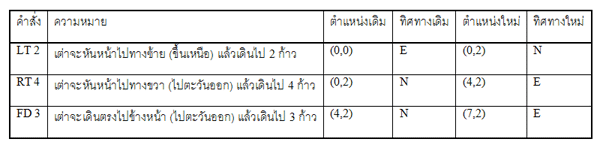
\includegraphics[width=0.9\textwidth]{../latex/img/1018/1018-1.png}
\end{figure}

อย่างไรก็ตาม เต่าจะอยู่ได้ในพิกัดที่มีค่าเป็นจำนวนเต็มเท่านั้น และเต่าจะอยู่ในบริเวณ $-50\,000 \leq x \leq 50\,000$ และ $-50\,000 \leq y \leq 50\,000$ และถ้าเต่าได้รับคำสั่งให้เดินมามาแตะหรือข้ามขอบ เต่าจะตายก่อนที่จะเริ่มเดินและไม่มีการทำคำสั่งที่เหลือต่อ และถ้าเต่าได้รับคำสั่งให้เดินมามาแตะหรือข้ามขอบ เต่าจะตายก่อนที่จะเริ่มเดินและไม่มีการทำคำสั่งที่เหลือต่อ

\bigskip
\underline{\textbf{โจทย์}} จงเขียนโปรแกรม เพื่อรับคำสั่งเพื่อควบคุมเต่ามาปฏิบัติ หลังจากปฏิบัติตามคำสั่งแล้วให้ระบุว่า เต่าจะอยู่ในตำแหน่งใดและมุ่งหน้าไปในทิศทางใด การเริ่มต้นของเต่าอยู่ที่พิกัด $(0,0)$ และหันหัวไปทางทิศตะวันออกเสมอ

\InputFile

\textbf{บรรทัดแรก} รับจำนวนเต็ม $n$ แทนจำนวนคำสั่งทั้งหมด โดย $0 < n < 10\,000$

\textbf{บรรทัดที่ $2$ ถึง $n+1$} บรรทัดที่ $i+1$ ให้รับคำสั่งที่ $i$ โดยที่คำสั่งจะอยู่ในรูปแบบ $c$ $k$ (คั่นด้วยช่องว่าง $1$ ช่อง)โดยที่ค่าของ $c$ ที่จะเป็นได้คือ \textbf{FD RT LT BW} และ $0 \leq k \leq 50\,000$

\OutputFile

\textbf{บรรทัดแรก }ถ้าเต่าตายให้แสดงคำว่า DEAD ถ้าเต่าไม่ตายให้แสดงพิกัด $(x,y)$ สุดท้ายหลังจากที่ชุดคำสั่งสิ้นสุด

\textbf{บรรทัดที่สอง} ถ้าเต่าตายไม่ต้องแสดงผลลัพธ์ใด ๆ ถ้าเต่าไม่ตายให้แสดงทิศทางที่เต่าหันหัวไป โดย N S E W จะแทนทิศเหนือ ใต้ ตะวันออก และตะวันตก ตามลำดับ

\Examples

\begin{example}
\exmp{3
LT 2
RT 4
FD 3}{7 2
E}%
\exmp{2
BW 50000
FD 4}{DEAD}%
\end{example}


\Source

การแข่งขันคณิตศาสตร์ วิทยาศาสตร์ โอลิมปิกแห่งประเทศไทย สาขาวิชาคอมพิวเตอร์ ประจำปี 2547

\end{problem}

\end{document}